\documentclass[tikz,border=6pt]{standalone}
\usepackage{fontspec}
\setmainfont{Noto Sans}
\usepackage{amsmath}
\usepackage{tikz}
\usetikzlibrary{arrows.meta,positioning}
\definecolor{cudaG}{RGB}{118,185,0}
\definecolor{sadRed}{RGB}{200,60,50}
\definecolor{gsBlue}{RGB}{40,110,190}
\definecolor{pyYel}{RGB}{240,170,30}
\definecolor{secG}{RGB}{85,85,85}
\begin{document}
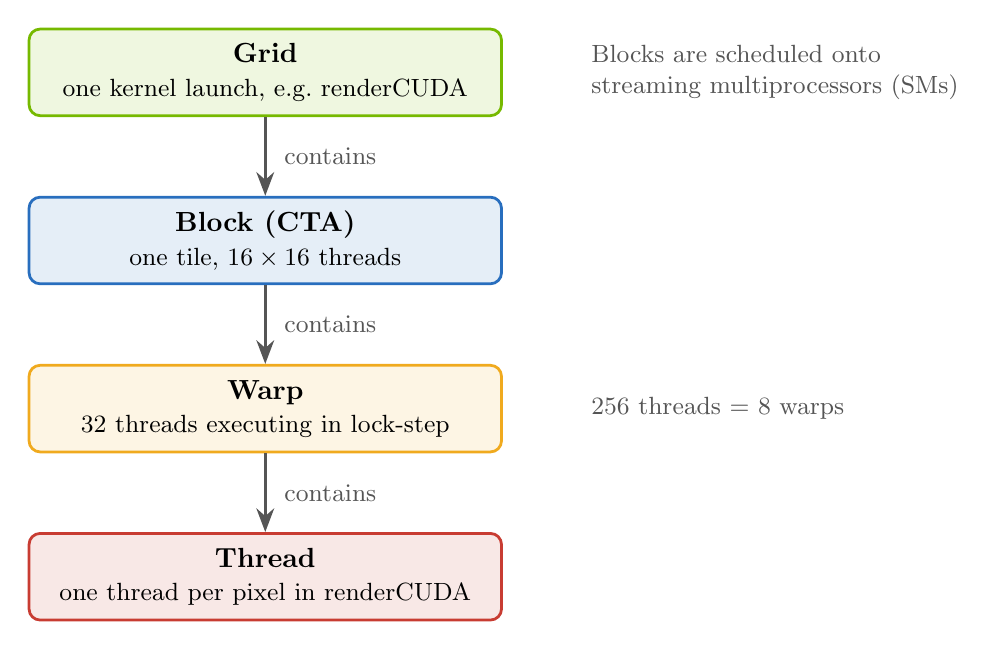
\begin{tikzpicture}[font=\sffamily]
  \tikzset{lvl/.style={draw=#1,line width=1pt,rounded corners,fill=#1!12,minimum width=6.0cm,minimum height=1.1cm,align=center,font=\normalsize}}
  \node[lvl=cudaG] (grid) at (0,0) {\textbf{Grid}\\{\small one kernel launch, e.g.\ renderCUDA}};
  \node[lvl=gsBlue,below=1.0cm of grid] (block) {\textbf{Block (CTA)}\\{\small one tile, $16\times16$ threads}};
  \node[lvl=pyYel,below=1.0cm of block] (warp) {\textbf{Warp}\\{\small 32 threads executing in lock-step}};
  \node[lvl=sadRed,below=1.0cm of warp] (thr) {\textbf{Thread}\\{\small one thread per pixel in renderCUDA}};
  \foreach \a/\b in {grid/block,block/warp,warp/thr} {
    \draw[-{Stealth[length=3mm]},line width=1.2pt,secG] (\a) -- node[right=3pt,font=\small,secG] {contains} (\b);
  }
  \node[right=1.0cm of grid,align=left,font=\small,secG] {Blocks are scheduled onto\\streaming multiprocessors (SMs)};
  \node[right=1.0cm of warp,align=left,font=\small,secG] {256 threads = 8 warps};
\end{tikzpicture}
\end{document}
